\documentclass{article}
\usepackage[utf8]{inputenc}
\usepackage{amsmath}
\usepackage{amsthm}
\usepackage{graphicx}
\usepackage{hyperref}
\usepackage{geometry}
\geometry{a4paper, portrait, margin=1in}

\usepackage{geometry}
\geometry{a4paper, portrait, margin=1in}

\theoremstyle{plain}
\newtheorem{thm}{Theorem}

\theoremstyle{definition}
\newtheorem{defn}{Definition} % definition numbers are dependent on theorem numbers
\newtheorem{exmp}{Example} % same for example numbers

\title{Computer Networks (UE18CS301)\\
 \large Unit 1
 }
\author{Aronya Baksy}
\date{August 2020}

\begin{document}

\maketitle

\section{Introduction}
\begin{defn}
    A \textbf{Computer Network} can be defined as $\geq 2$ computing devices connected to each other capable of sharing information between them.
\end{defn}

\section{The Internet}

The internet is a network of computer networks. It consists of traditional devices (PCs, Workstations, servers) and non-traditional IoT devices (TVs, gaming consoles, home security appliances, cars, smart speakers etc.) connected to each other via a well-defined communication protocol called TCP/IP. 

\subsection{The nuts-and-bolts description}

The following components comprise the internet according to the nuts and bolts description: 

\begin{enumerate}
    \item \textbf{End Systems:}
        \begin{enumerate}
            \item These are also known as \textbf{Edge Systems} or \textbf{hosts}.
            
            \item They run network applications at the end points/edges of the internet 
            
            \item eg: PCs, smartphones, Servers, IoT devices
        \end{enumerate}
        
    \item \textbf{Packet Switches:}
        \begin{enumerate}
            \item Forward packets, ie. chunks of data from one point in the internet to the next
            
            \item \textbf{Routers} are Level 3 communication devices, as they act on level 3, ie. the \textbf{network} layer of the TCP/IP model. They are used in the network core.
            
            \item \textbf{Switches} are Level 2 communication devices, as they act on level 2, ie. the \textbf{data link} layer of the TCP/IP model. They are used in access networks.
        \end{enumerate}
    
    \item \textbf{Communication Links:}
        \begin{enumerate}
            \item The hardware media needed to transfer data between end systems and the packet switches
            
            \item These comprise of cables (copper/fiber optic), radio and satellite communication
        \end{enumerate}
    
    \item \textbf{ISPs}
    \begin{enumerate}
        \item ISPs provide connections between end systems and the internet
        
        \item An ISP in itself is a network of packet switches and communication links.
    \end{enumerate}
    
    \item \textbf{Protocols:}
    \begin{enumerate}
        \item A protocol can be defined as a set of rules or standards used to define the methods and formats for sending/receiving of messages.
        
        \item The 2 most common protocols in use as part of the internet are \textbf{TCP} (Transmission Control Protocol) and \textbf{IP} (Internet Protocol)
        
        \item The IP protocol specifies the format of the packets that are sent and received among routers and end systems.
        
        \item Other protocols in use by the internet are FTP (File Transfer Protocol), SMTP (Simple Mail Transfer Protocol), HTTP (HyperText Transfer Protocol), UDP (User Datagram Protocol)
    \end{enumerate}
    
    \item \textbf{Internet Standards:} 
    \begin{enumerate}
        \item These are the definitions for the protocols that define the functioning of the internet.
        
        \item They are defined in the form of documents called \textbf{RFCs} (Request for Comments) that are sent out by the \textbf{IETF} (Internet Engineering Task Force) 
        
        \item The IETF is responsible for defining protocols such as TCP, IP, SMTP, HTTP etc.
        
        \item Other bodies such as the \textbf{IEEE} (International association for Electrical and Electronics Engineers) define standards for communication protocols like WiFi and Ethernet (IEEE 802)
    \end{enumerate}
\end{enumerate}

\begin{figure}[h]
    \centering
    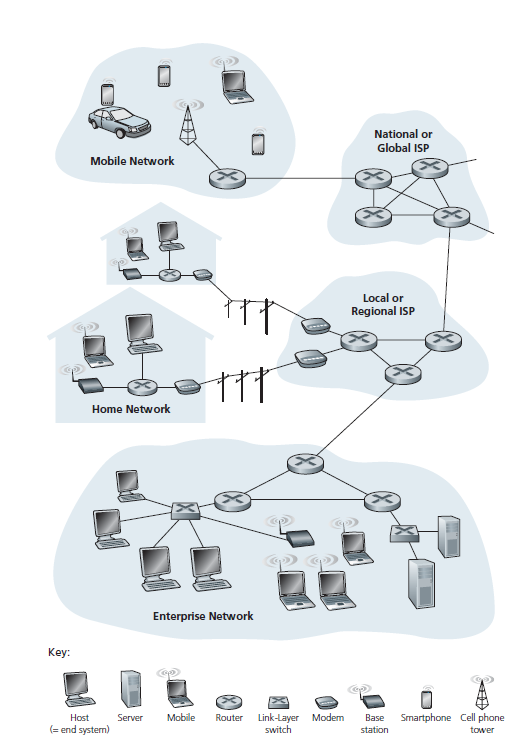
\includegraphics{cn1.png}
    \caption{A schematic computer network}
    \label{fig:my_label}
\end{figure}

\subsection{The services description}
\begin{itemize}
    \item The internet may also be viewed from the application programmer's point of view as a service, that offers methods to transmit user data from one end system to another.
    
    \item The end systems offer \textbf{APIs} (Application Programming Interfaces) as \textbf{Hooks} into the internet ecosystem. The application developer can use these hooks to plug their application into the internet, and use the internet to transfer data.
    
    \item The internet API is a standard that specifies how a program running on one end system asks the Internet infrastructure to deliver data to a specific destination program running on another end system.
    
    \item The internet, in this point of view, can be considered to be analogous to a postal system, where the sender of the letter (the programmer) can use the post office (the API) as a \textbf{hook} into the postal service that transfers the letter to the final receiver. 
\end{itemize}

\section{Protocols}

\begin{defn}
    A protocol defines the format and order of messages sent and received between two or more communicating entities, as well as the action to be taken on the transmission and/or the receipt of messages or any other event. 
\end{defn}

\begin{figure}[h]
    \centering
    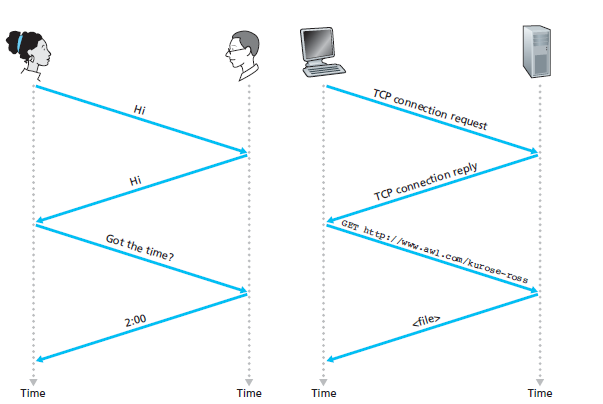
\includegraphics{cn3.png}
    \caption{Human communication protocol and HTTP Protocol}
    \label{fig:my_label_2}
\end{figure}
Some of the protocols are listed below along with the layers of the 7-layer OSI Reference Model in which they function.

\begin{enumerate}
    \item \textbf{Application Layer:} DNS, WWW/HTTP, P2P, email/POP, SMTP, FTP, telnet
    
    \item \textbf{Presentation Layer:} HTML, DOC, JPEG, AVI, Socket
    
    \item \textbf{Session Layer:} Session establishment in TCP, SIP, UDP
    
    \item \textbf{Transport Layer:} TCP, UDP, SSL, TLS, SCTP
    
    \item \textbf{Network Layer:} IP, ARP, Routing Protocols like OSPF, EIGRP
    
    \item \textbf{Data Link Layer:} Ethernet, IEEE 802.11, MAC/LLC
    
    \item \textbf{Physical Layer:} RJ45, RS-232
\end{enumerate}
\section{The Network Edge: client-server architecture}
\begin{itemize}
    \item The network edge is primarily comprised of end systems (see above for definition of an end system).
    
    \item End systems are also referred to as \textbf{hosts} as they are responsible for \textit{hosting} the application software that communicates with the internet
    
    \item End systems (or hosts) may be further subdivided into \textbf{client} and \textbf{server} machines.
    
    \item Informally, a client machine is one that requests data that is stored on a server. Client machines are low performance machines like PCs, mobiles, tablets, and non-traditional IoT devices.
    
    \item A server, in comparison, is a more powerful machine that is capable of servicing multiple client requests and handling very complicated processing of queries, while storing large amounts of data.
    
    \item Servers today appear in large clusters called \textbf{data centers}. (\url{https://cloud.google.com/about/locations} gives a rough idea about the number of Google Data Centers)
\end{itemize}

\subsection{Access Networks}
\begin{defn}
    An \textbf{access network} is a network that connects an edge system to the first router in the path from that end system to any other distant system, also called the \textit{edge router}
\end{defn}

\subsubsection{Home Connection: DSL}

\begin{itemize}
    \item \textbf{DSL} (Digital Subscriber Line) is one of the most popular methods for homes to connect to the internet. This service is provided by telephone companies. 
    
    \item Each customer's DSL Modem uses the same cable as the telephone line (twisted pair copper cable) to exchange data with a DSL Access Multiplexer (\textbf{DSLAM}) 
    
    \item The DSL modem converts digital data (represented as 0/1) into high frequency tones that can be transferred over the telephone line. The residential telephone line carries both data and traditional telephone signals
    simultaneously, which are encoded at different frequencies:
    
    \begin{itemize}
        \item A high-speed downstream (internet to home) channel (50kHz - 1MHz band)
        
        \item A medium-speed upstream (home to internet) channel (4kHz - 50kHz band)
        
        \item An ordinary two-way channel (0-4kHz)
    \end{itemize}
    
    \item On the customer side, a splitter separates the data and telephone signals arriving to the home and forwards the data signal to the DSL modem.
    
    \item On the telephone operator's side, in the Central Office, the DSLAM separates the data and phone signals and sends the data into the Internet.

\begin{figure}[h]
    \centering
    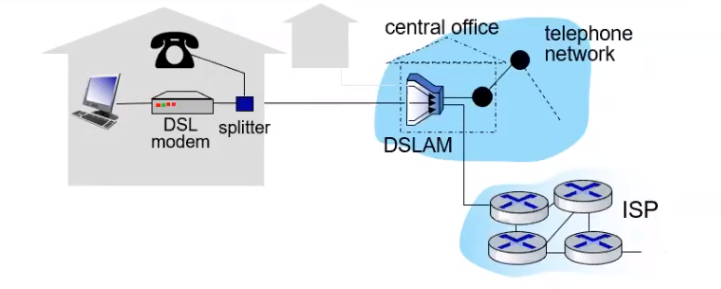
\includegraphics[scale=0.8]{cn2.png}
    \caption{DSL Internet Access}
    \label{fig:my_label_3}
\end{figure}
\end{itemize}

\subsubsection{Home Connection: Cable}
\begin{itemize}
    \item Cable internet shares IP data and cable television data over a common channel. 
    
    \item Fiber optics connect the cable head end to neighborhood-level junctions, from which traditional coaxial cable is then used to reach individual houses and apartments.
    
    \item At the Cable head end, the CMTS (Cable Modem Termination System) serves the role of turning the analog signal sent from the cable modems in many downstream homes back into digital format.
    
    \item One important characteristic of cable Internet access is that it is a shared broadcast medium. In particular, every packet sent by the head end travels downstream on every link to every home and every packet sent by a home travels on the upstream channel to the head end.
\end{itemize}

\begin{figure}[h]
        \centering
        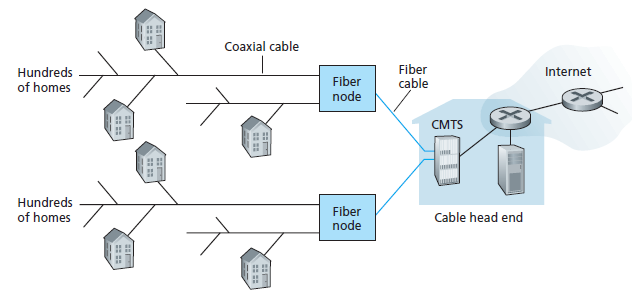
\includegraphics{cn4.png}
        \caption{Cable Internet Access}
        \label{fig:my_label_4}
    \end{figure}

\begin{itemize}
    \item One common feature of Cable and DSL is the asymmetric access, where the download and upload speeds are different.
    
    \item For DSL, 24 Mbps downstream, 2.5 Mbps upstream
    
    \item For Cable, 42.8 Mbps downstream, 30.7 Mbps
\end{itemize}
\subsubsection{Enterprise connection: Ethernet and WiFi}

\begin{itemize}
    \item In corporate/educational settings, LAN (Local Area Network) is used to connect the end systems to the edge routers. 
    
    \item \textbf{Ethernet} users use twisted pair copper wire to connect to an Ethernet switch, which in turn connects to the larger internet. 
    
    \item Ethernet offers users 100 Mbps access to the internet, while servers have 1-10 Gbps access.
    
    \item\textbf{WLAN (Wireless LAN)} is a method for wirelessly connecting mobile devices in an enterprise environment. 
    
    \item A WLAN user must be within a few tens of meters from a WLAN access point. Wireless access is based on the IEEE 802.11 b/g/n/ac protocols, commonly called WiFi.
    
    \item WiFi offers transmission rates of 11, 54 or 450 Mbps.
    
    \item Outside the enterprise context, many homes combine broadband residential access (that is, cable modems or DSL) with these inexpensive wireless LAN technologies to create powerful home networks. 
    
    \item This home network consists of a roaming laptop as well as a wired PC; a base station (the wireless access point), which communicates with the wireless PC; a cable modem, providing broadband access to the Internet; and a router, which interconnects the base station and the stationary PC with the cable modem.
\end{itemize}

\begin{figure}[h]
    \centering
    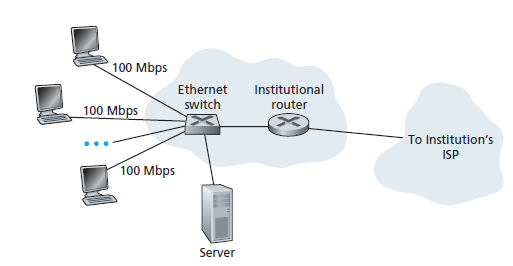
\includegraphics{cn5.png}
    \caption{Ethernet Internet Access}
    \label{fig:my_label_5}
\end{figure}

\section{Physical Communication Media}

\begin{itemize}
    \item For each transmitter-receiver pair, the bit is sent by propagating electromagnetic waves or optical pulses across a physical medium. The physical medium can take many shapes and forms and does not have to be of the same type for each transmitter-receiver pair along the path.
    
    \item Physical media fall into two categories: guided media and unguided media.
    
    \item With \textbf{guided media}, the waves are guided along a solid medium, such as a fiber-optic cable, a twisted-pair copper wire, or a coaxial cable.
    
    \item With \textbf{unguided media}, the waves propagate in the atmosphere and in outer space, such as in a wireless LAN or a digital satellite channel.
\end{itemize}

\subsection{Twisted Pair Copper Wire}

\begin{itemize}
    \item Twisted pair consists of two insulated copper wires, each about 1 mm thick, arranged in a regular spiral pattern. 
    
    \item The wires are twisted together to reduce the electrical interference from similar pairs close by.
    
    \item One pair constitutes one communication link. A number of pairs are typically bundled together in a protective shield (\textbf{Shielded Twister Pair} Cable)
    
    \item LANs use \textbf{Unshielded Twisted Pair (UTP)} cables, for intra building communication as an example. Shielded Twisted Pair cables are more expensive and have less attenuation rate. 
    
    \item Cat 5: upto 100 Mbps, or 1 Gbps over an Ethernet connection
    
    \item Cat 6: upto 10 Gbps over Ethernet

\end{itemize}

\subsection{Coaxial Cable}
\begin{itemize}
    \item Concentric (not parallel, as in the case of twisted pair) copper conductors. 
    
    \item With special insulation, shielding and this construction, coaxial cables achieve high data transmission rates.
    
    \item They are used primarily in cable TV systems, and can be coupled with cable modems to provide residential internet access at tens of Mbps. 
    
    \item The transmitter shifts the digital internet signal to a specific frequency band, which is sent to one or more receivers. 
    
    \item Coaxial cables can also be used as a shared medium, with a number of end systems conneced to the same cable. 
\end{itemize}

\subsection{Fiber Optic Cable}
\begin{itemize}
    \item A thin flexible medium that conducts data via pulses of light, with each pulse representing one bit of information. 
    
    \item A single fiber can support upto 100s of gigabits per second (Gbps). 
    
    \item They are immune to electromagnetic interference, have very low signal attenuation upto 100km, and are almost impossible to tap. 
    
    \item The high cost of fiber optic network devices (transmitters, receivers, switches) has meant reduced adoption for short haul networks like LAN or residential access networks. 
    
    \item The OC-$n$ (Optical Carrier) standards define the link speeds for certain standard fiber optic configurations; the link speed is calculated as $n \times 51.8$ Mbps. Standards in use today include OC-1, OC-3, OC-12, OC-24, OC-48, OC-96, OC-192 and OC-768. 
\end{itemize}

\subsection{Terrestrial Radio Channels}
\begin{itemize}
    \item Radio waves carry signals in the radio part of the electromagnetic spectrum. 
    
    \item Radio communication does not need a physical medium to be installed, can penetrate walls, can provide connectivity to mobile users and can carry signals for large distances. 
    
    \item Radio wave characteristics are significantly influenced by the environmental factors. These are parameterized by the \textbf{path loss} and \textbf{shadow fading} (reduce signal strength as the signal travels over or around objects), \textbf{multi-path fading} (due to signal reflection) and \textbf{interference} (due to other EM signals and transmissions). 
\end{itemize}

\subsection{Satellite Radio Channels}
\begin{itemize}
    \item A communication satellite links two or more Earth-based microwave transmitter/ receivers, known as ground stations. 
    
    \item The satellite receives transmissions on one frequency
band, regenerates the signal using a repeater (discussed below), and transmits
the signal on another frequency. 

    \item Two types of satellites are used in communications: \textbf{geostationary} satellites and \textbf{low-earth orbiting} (LEO) satellites.
\end{itemize}


\section{The Network Core}
\subsection{Packet Switching}

\begin{itemize}
    \item To send a message from a source end system to a destination end system, the source breaks the message into well-formatted chunks called \textbf{packets}. 
    
    \item Each packet travels through several communication links, and \textbf{packet switches} (ie. routers, link-layer switches).
    
    \item The packets are transmitted at the \textit{full} transmission rate of the link, hence for an end system/switch transmitting packets of length $L$ bits at a rate of R bits/sec, the time to transmit the packet would be 
    \begin{equation}
        T_{transmit} = \frac{L}{R}
    \end{equation}
\end{itemize}
    
\subsubsection{Store-and-Forward Transmission}
    \begin{itemize}
        \item Most packet switches use store-and-forward transmission at the inputs to the links.
        
        \item Store and forward transmission means that the entire packet must be received at the input before it can be propagated to the next element in the network. 
        
        \item The packet bits that a router receives are stored in the router's \textbf{buffer} until the entire packet is received, then the packet can be transmitted and the buffer can be cleared. 
        
        \begin{figure}[h]
            \centering
            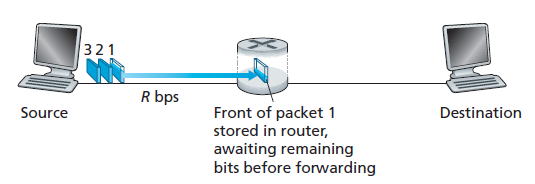
\includegraphics{cn6.png}
            \caption{Store-and-Forward Packet Switching}
            \label{fig:my_label_6}
        \end{figure}
        
        \item In the example above, when packet 1 is completely received by the router, it can be forwarded and simultaneously the bits of packet 2 start getting transmitted by the router. By the time packet 1 fully reaches the destination, packet 2 is fully at the router. 
        
        \item For a single packet of length $L$ bits, travelling over $N$ communication links (hence $N-1$ routers), each having a transmission rate of $R$ bits/sec, the end to end delay between source and destination is 
        \begin{equation}
            d_{end-to-end} = N \frac{L}{R}
        \end{equation}
        
        \item Generalizing this to $P$ packets being transmitted, we have
        \begin{equation}
            d_{end-to-end} = (N+P-1)\frac{L}{R}
        \end{equation}
        
        In the given example, we have $N=2$ and $P=3$, hence the end to end transmission delay is $4\frac{L}{R}$.
    \end{itemize}
    
    \subsubsection{Queuing delays and Transmission Loss}
    \begin{itemize}
        \item For each input link into a router, the router maintains an \textbf{output buffer} (or an output queue) that stores the the packets that the router is about to send into the output link.
        
        \item If an arriving packet arrives while the link is already busy transmitting another packet, then it must wait until the link is free. 
        
        \item This leads to an addition \textbf{queuing delay} in addition to the store and forward delay described above. 
        
        \item If the arriving packet finds that the buffer is full, then either the arriving packet or one of the packets in the queue must be dropped to make space. This leads to \textbf{packet loss}.
        
        \item This situation normally occurs when the speed of the input links are higher than the speed of the output link, as shown in the figure below (Figure 7).
    \end{itemize}
    
    \subsubsection{Forwarding tables and Routing Protocols}
    \begin{itemize}
        \item When a router arrives at a packet, the router consults its forwarding table using a part of the destination address of the packet (its \textbf{IP Address}) to direct the packet to its appropriate outbound communication link. 
        
        \item Forwarding tables are set using an automated approach that uses a routing algorithm (static or dynamic) to determine the shortest path between a given source and a destination. (eg: Dijkstra's Algorithm)
    \end{itemize}
    
    \begin{figure}[ht]
        \centering
        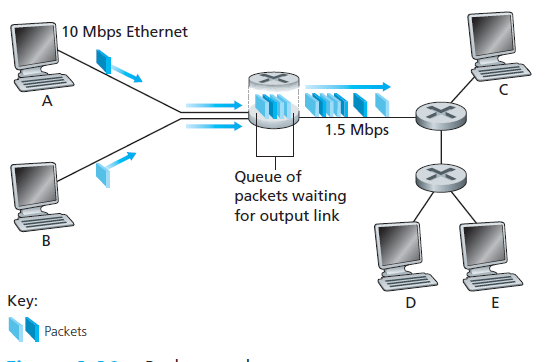
\includegraphics{cn7.png}
        \caption{Queuing delay in Packet Switching}
        \label{fig:my_label_7}
    \end{figure}
    
\subsection{Circuit Switching}
\begin{itemize}
    \item In a circuit-switched network, all resources (buffers, link transmission rate) along a path are allocated and \textbf{reserved} for the entire duration of the communication between source and destination. 
    
    \item In packet-switched networks, by contrast, these resources are used on demand, and hence packets may have to wait until the resource is available to actually make use of it (leading to queuing delays and end-to-end transmission delays as described above). 
    
    \item Before any communication can happen, a connection must be established between the two parties. This is a \textit{bonafide} connection, meaning that all the network devices along the connection must maintain the same state for the entire duration of the communication. 
    
    \item In the parlance of telephone networks, such an end-to-end connection is called a \textit{circuit}, hence the name circuit switching is given to such a system. 
    
    \item Along with the path and the network devices, a constant fraction of the transmission link's capacity must also be reserved for the duration of the connection. This guarantees the data transfer at a  \textit{guaranteed} constant rate for the entire communication. 
    
    \item The splitting of the link capacity between each circuit is achieved using either\textbf{ Time Division Multiplexing (TDM)} or \textbf{Frequency Division Multiplexing (FDM)}.
\end{itemize}

\subsubsection{Frequency Division Multiplexing (FDM)}
\begin{itemize}
    \item The frequency spectrum of a link is split up for each connection across that link.
    
    \item The link dedicates a frequency band to each connection for the duration of the connection.
\end{itemize}

\subsubsection{Time Division Multiplexing (TDM)}
\begin{itemize}
    \item Time is divided into frames, and each frame is subdivided into slots. 
    
    \item When the network establishes a connection across a link, the network dedicates one time slot in every frame to this connection. These slots are dedicated for the sole use of that connection, with one time slot available for use (in every frame) to transmit the connection’s data.
    
\end{itemize}

\begin{figure}[ht]
    \centering
    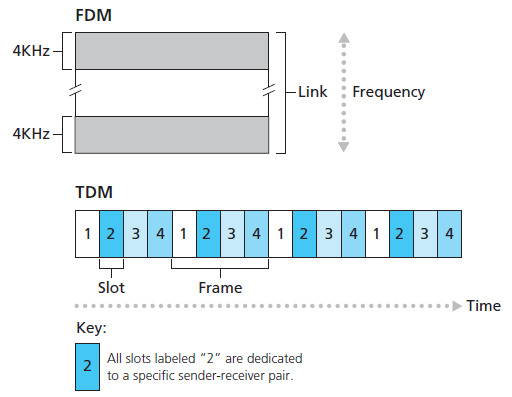
\includegraphics{cn8}
    \caption{FDM and TDM in a circuit-switched network}
    \label{fig:my_label_8}
\end{figure}

\subsection{Comparison between Packet and Circuit Switching}
\begin{itemize}
    \item Circuit Switching may lead to under utilization of resources during silent periods. 
    
    \item For example, if one person on a telephone call stops talking, the idle resources (time/freq bands) cannot be used by any other connections along the same link. 
    
    \item Establishing end-to-end circuits and reserving end-to-end transmission capacity is complicated and requires complex signaling software to coordinate the operation of the switches along the end-to-end path.
    
    \item Suppose users share a 1 Mbps link, and users are active for 10\% of time, and inactive for 90\% of time. While the user is active, the user generates data at a rate of 100 kbps. 
    
    \item In a circuit switched network, 100 kbps of link capacity must be reserved for all users at all points in time. This implies that with a total link capacity of 1 Mbps as mentioned, only 10 users can simultaneously use a circuit switched network. 
    
    \item In a packet switched network, assuming that the total number of users is 35, the probability of having 10 simultaneous active users on the network is 0.9996, and the network functions exactly at the same performance as a circuit switched network. 
    
    \item When there are 11 or more active users, the router buffer queue begins to expand as the aggregate arrival rate of packets exceeds the output capacity of the link, and the output queue will begin to grow (it grows until the aggregate input arrival rate of packets drops below 1 Mbps). However with 35 total users, the probability of having $\geq$ 11 users is only 0.0004, which is very small. 
    
    \item In conclusion, the packet switched network offers similar performance to a circuit switched network while allowing almost thrice as many total users. 
\end{itemize}

\section{Network of Networks: Interconnection of ISPs}
\subsection{Network Structure 1} 
\begin{itemize}
    \item This is a global ISP that connects all the individual access networks. This network would span the entire globe and contain at least one router near each access network. 
    
    \item This single global ISP would charge each local access ISP according to the volume of traffic in the link between the global and local ISPs. The access ISP is called a \textbf{customer} and the global ISP is called the \textbf{provider}.
\end{itemize}
    
\subsection{Network Structure 2} 
\begin{itemize}
    \item 
    This consists of multiple global ISPs that connect a large number of local access ISPs. These multiple global ISPs must themselves be connected to ensure full connectivity among all the local access ISPs.
    
    \item This structure is more favourable for local access ISPs as they can choose between these global ISPs based on their pricing and infrastructure plans. 
\end{itemize}

\subsection{Network Structure 3}
\begin{itemize}
    \item Network Structure 2, just described, is a two-tier hierarchy with global transit providers residing at the top tier and access ISPs at the bottom tier. 

    \item In any given region, there may be a \textbf{regional ISP} to which the access ISPs in the region connect. Each regional ISP then connects to \textbf{tier-1 ISP}s.
    
    \item There may be multiple competing networks at each level of this hierarchy (regional, tier-1), and there may be further subdivisions of this hierarchy, such a country-wide larger regional ISP that connects multiple regional ISPs, and itself connects to the tier-1 ISP (eg: in China). 
    
    \item Such a multi-tier architecture is Network Structure 3. At each level there is a customer-provider relationship where the customer pays the provider for the service they provide. 
\end{itemize}

\subsection{Network Structure 4}
\begin{itemize}
    \item To the idea of network structure 3, some devices, namely \textbf{PoP}s (Points of Presence), \textbf{multi-homing}, \textbf{peering} and \textbf{IXP}s (Internet eXchange Points) must be added to make it more accurate to the structure of the current internet. 
    
    \item A PoP is a group of one or more routers (at the same location) in the provider’s network where customer ISPs can connect into the provider ISP. For a customer network to connect to a provider’s PoP, it can lease a high-speed link from a third-party telecommunications provider to directly connect one of its routers to a router at the PoP
    
    \item Multi homing is a facility that allows a customer ISP to connect to multiple providers in the level immediately above, or even levels above that. (eg: an access ISP cann connect to multiple regional ISPs, or multiple regional ISPs along with a direct link to a tier-1 ISP). This is a method of building fault tolerance into an access network.
    
    \item Peering is a method of directly connecting two ISPs which are at the same level of the hierarchy, instead of connection via a higher level provider. This connection is commonly done out of mutual interest and no ISP pays the other for a peering link. 
    
    \item An IXP is an infrastructure built by a third-party company. It is a meeting point where multiple ISPs can peer together, and it consists of multiple link-layer switches connected within a single building. 
\end{itemize}

\subsection{Network Structure 5}
\begin{itemize}
    \item In addition to the structure defined in Network Structure 4, the modern internet contains one final piece, the \textbf{content delivery netowrk}.
    
    \item Such networks are maintained by content providers (such as Google and its related services like YouTube, Drive, Google Office Suite, etc.)
    
    \item A CDN has its own internal network by which all the data centers and servers in the CDN can communicate with each other. 
    
    \item CDNs connect to the rest of the internet either by directly connecting to tier-1 ISPs or directly peering with the lower levels using peering networks or at IXPs.
\end{itemize}
\begin{figure}
    \centering
    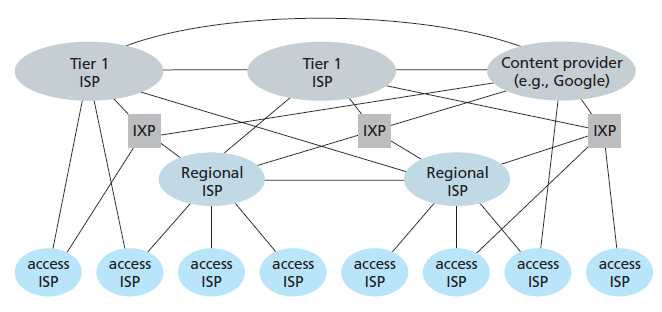
\includegraphics{cn9.png}
    \caption{Interconnection of ISPs}
    \label{fig:my_label_9}
\end{figure}

\section{Delay, Loss and Throughput in Computer Networks}
As a packet travels from one node (router) to the next in the network, it faces 4 main types of delays: \textbf{nodal processing delays}, \textbf{queuing delay}, \textbf{transmission delay} and \textbf{propagation delay}.

\subsection{Types of Delays}

\subsubsection{Nodal Processing Delay}
\begin{itemize}
    \item This is the delay involved in reading the packet header, and routing the packet to its appropriate link, as well as the delays involved in checking for bit-level errors in the packet.
    
    \item After the nodal processing, the packet is directed to a queue where it waits for transmission.
    
    \item In a modern router, this delay is on the order of microseconds. 
\end{itemize}

\subsubsection{Queuing Delay}
\begin{itemize}
    \item The queuing delay is the time spent by the packet inside the router buffer, waiting to be transmitted on the outbound link. 
    
    \item If the queue is empty and no other packets are transmitted on the link, the queuing delay is 0. If incoming traffic is heavy, and lots of packets are waiting to be transmitted, this leads to significant queuing delays.
    
    \item Queuing delays are on the order of micro or milliseconds. 
\end{itemize}

\subsubsection{Transmission Delay}
\begin{itemize}
    \item This is the time taken to push all the bits of the packet from the router onto the link.
    
    \item If the packet is $L$ bits long, and $R$ is the transmission rate of the link (in bps), then the transmission delay is given by 
    
    \begin{equation}
        d_{trans} = \frac{L}{R}
    \end{equation}
    
    \item Transmission delays are on the order of micro or milliseconds.
\end{itemize}

\subsubsection{Propagation Delay}
\begin{itemize}
    \item The delay involved in propagating all the packet bits from the beginning of the link to the next router.
    
    \item This is given by
    
    \begin{equation}
        d_{prop} = \frac{d}{s}
    \end{equation}
    
    Where $d$ is the length of the link, and $s$ is the propagation speed of the link (in m/s)
    
    \item These are on the order of milliseconds. 
\end{itemize}

\subsection{Queuing Delay and Packet Loss}

\begin{itemize}
    \item The queuing delay, unlike the other three types of delays, may vary from packet to packet, depending on the prevailing conditions of the queue and the outbound link.
    
    \item Let $a$ denote the rate of packet arrival at the router buffer, and $L$ denote the packet length in bits. Therefore the rate of arrival of bits at the router buffer is $La$ bps.
    
    \item If $R$ is the link transmission rate in bps, then the ratio $La/R$, called the \textbf{traffic intensity} is a good estimate of the queuing delay. 
    
    \item If $La/R > 1$ then the rate of incoming bits exceeds the rate of outgoing bits. Thus the queue grows without bound, and the queuing delay approaches infinity.
    
    \item If $La/R \leq 1$ then the nature of packet arrival affects the queuing delay. Uniform rate of packet arrival leads to zero queuing delay, but packet arrival in large bursts may lead to large avg queuing delays. 
\end{itemize}

\begin{figure}[h]
    \centering
    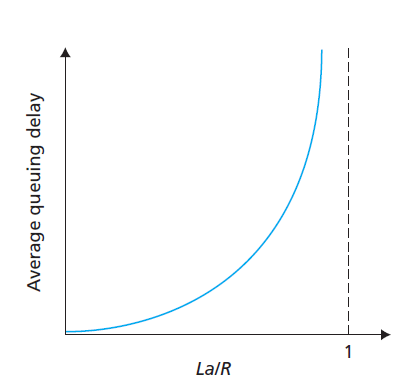
\includegraphics{cn10.png}
    \caption{Dependence of avg queuing delay on traffic intensity}
    \label{fig:my_label_10}
\end{figure}

\section{Protocol Layers and Layered Architecture of the Internet}
\begin{itemize}
    \item The internet and its associated hardware infrastructure are organized as layers so that they can be easily understood and studied.
    
    \item These protocol \textbf{layers} are organized in a stack, with each layer providing service to the layers above it, and being independent of the layers below it. 
    
    \item Layering offers the advantages of \textbf{modularity} (which helps in isolating faults and updating hardware) and a clear \textbf{standard structure} for vendors to implement.
    
    \item The disadvantages of layering are \textbf{duplication} of services in more than one layer, and the possible \textbf{dependence} of layers on information from other layers.
\end{itemize}
\begin{figure}
    \centering
    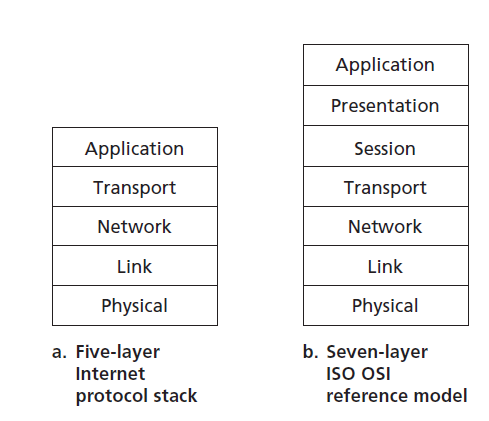
\includegraphics{cn11.png}
    \label{fig:my_label_11}
\end{figure}

\subsection{Internet Protocol Stack}
\subsubsection{Layer 5: Application Layer}
\begin{itemize}
    \item \textbf{Network applications} and their associated protocols reside in this layer.
    
    \item Application layer protocols include \textbf{HTTP} (to receive and transfer web documents across the internet), \textbf{SMTP} (e-mail transfer), \textbf{FTP} (file transfer between end systems) and \textbf{DNS} (translation of human-readable web addresses to 32-bit IPv4 addresses). 
    
    \item End systems use the application layer to exchange information in the form of \textbf{messages}.
\end{itemize}

\subsubsection{Layer 4: Transport Layer}
\begin{itemize}
    \item This layer provides support to transfer messages between application endpoints. 
    
    \item The primary protocols in this layer are \textbf{TCP} (a connection oriented service that guarantees reliable data transfer, offers congestion and flow control, along with the breaking of large messages into shorter blocks), and \textbf{UDP} (a connectionless, no frills service without congestion/flow control and no guarantee of reliable tranmission, but high speed and stateless).
    
    \item Transport layer protocols break the messages from the application layer into smaller blocks called \textbf{segments}.
\end{itemize}

\subsubsection{Layer 3: Network Layer}
\begin{itemize}
    \item The network layer consists primarily of the IP protocol, that takes in a transport layer segment along with a destination IP Address, and encapsulates this information into a structure called a \textbf{datagram}.
    
    \item The IP protocol defines the structure and format of the datagrams, as well as many different routing protocols that determine the routes to be followed by datagrams from source to destination. 
\end{itemize}

\subsubsection{Layer 2: Data Link Layer}
\begin{itemize}
    \item Also simply called the link layer, this layer moves datagrams between consecutive routers on the path defined by the network layer protocols. 
    
    \item Protocols acting in this layer include IEEE 802.11, Ethernet, and PPP. A datagram may pass through many different protocols on each router-router link through its route. 
    
    \item Link layer packets are called \textbf{frames} and they contain additional information in the form of the MAC Address or the hardware address of the destination router. 
\end{itemize}

\subsubsection{Layer 1: Physical Layer}
\begin{itemize}
    \item This layer deals with bit level transfer of frames between network devices, across the different types of physical media present on these links.
    
    \item The protocols on this layer are dependent on the link medium, eg: Ethernet has separate sub protocols for twisted-pair, coaxial and fiber optic cable media. 
\end{itemize}

\subsection{OSI 7-layer Reference Model}
The 7 layer model refers to two additional layers which are not part of the internet protocol. In the Internet protocol, these services are commonly wrapped into the application layer and are implemented only if needed.
\subsubsection{Presentation Layer}
\begin{itemize}
    \item This layer allows application layer services to interpret the meaning of data and take appropriate actions.
    
    \item Services like encryption, compression and description (to aid in conversion between hardware formats) of data fall into this layer. 
\end{itemize}

\subsubsection{Session Layer}
\begin{itemize}
    \item This layer offers services for synchronization and delimiting data exchange, including checkpointing and recovery. 
    
    \item It allows information of different streams, perhaps originating from different sources, to be properly combined or synchronized.
\end{itemize}
\subsection{Encapsulation}
\begin{itemize}
    \item All network devices organize their hardware into layers, but not all devices implement all the layers in the Internet Protocol stack.
    
    \item Link-layer switches implement only layers 1 and 2, while routers implement layers 1,2 and 3 only. 
    
    \item Each layer adds some information to the packet coming from the layer below it, and while going down the layers, this information is removed and used.
    
    \item Every packet has a \textbf{header} and a \textbf{payload}. The header consists of the new information being added, and the payload is the packet from the previous layer. 
\end{itemize}
\begin{figure}[ht]
    \centering
    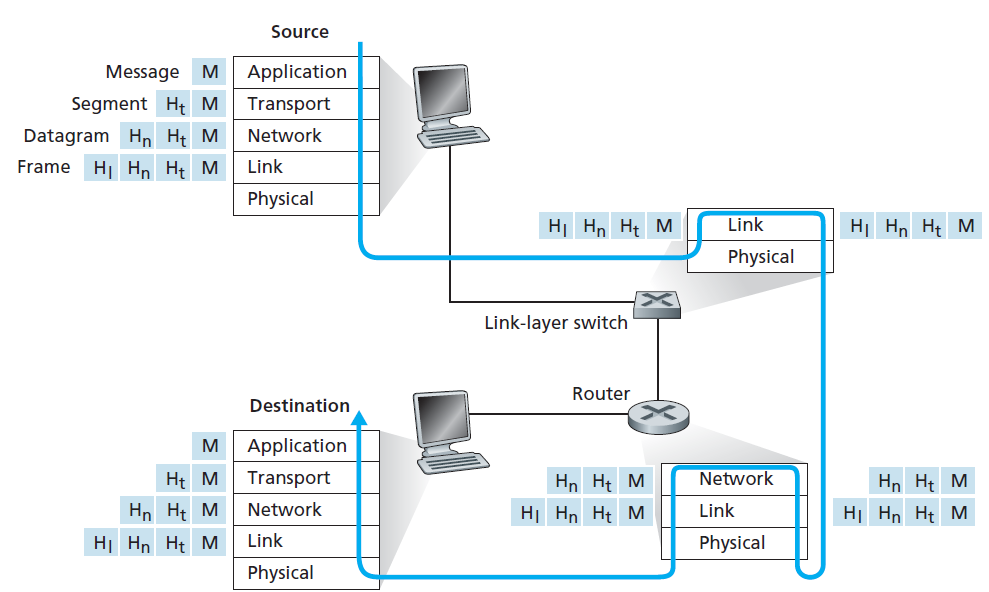
\includegraphics[scale=0.65]{cn12.png}
    \caption{Protocol Stacks on host systems, routers and link-layer switches}
    \label{fig:my_label_12}
\end{figure}

\begin{itemize}
    \item The application layer message $M$ is passed to the transport layer at the source
    
    \item The transport layers adds the information that is needed by the receiver side transport layer in the \textbf{transport layer header} $H_t$ (The port number). The combination of $M$ and $H_t$ is called the transport-layer \textbf{segment}.
    
    \item The transport-layer segment enters the network layer and the network-layer header $H_n$ is added to the segment (the IP Address of source and destination), making up the network-layer \textbf{datagram}.
    
    \item The datagram enters the link layer and the MAC address of the destination (contained in the header $H_l$) is added to it, turning it into the link-layer \textbf{frame}. 
    
    \item The frame is then transmitted over the physical layer.
\end{itemize}

\end{document}